\documentclass[10pt]{beamer}
%\documentclass[10pt, handout]{beamer}
%\usetheme{Madrid}
%\newlength{\pageheight}
%\setlength{\pageheight}{10cm}
%\usepackage{handoutWithNotes}
%\pgfpagesuselayout{2 on 1 with notes landscape}[a4paper,border shrink=5mm]

\usepackage[utf8]{inputenc}
\usepackage{dirtytalk}
\usepackage{amsmath}
\usepackage{amsfonts}
\usepackage{general}
\usepackage[cache=false]{minted}
\usepackage{booktabs}

\usepackage[nott]{inconsolata}

\DeclareMathOperator*{\argmax}{arg\,max}
%\DeclareMathOperator*{\argmin}{arg\,min}
\DeclareMathOperator*{\argmin}{\arg\min}

\definecolor{darkgreen}{rgb}{0.0, 0.5, 0.0}

\usepackage{pgf}
\usepackage{tikz}
\usetikzlibrary{arrows,automata}
\beamertemplatenavigationsymbolsempty

\addtobeamertemplate{title page}{
\includegraphics[scale=.5]{{../Images/UNAH-version-horizontal.png}}} %\hfill 
\includegraphics[scale=.3]{fabstracts2.png}}{}


%\titlegraphic{
%    \begin{tikzpicture}[overlay, remember picture]
%\node[at=(current page.north), anchor=north] {%
%    
\includegraphics[width=0.2\textwidth]{University_of_Pittsburgh_seal.png}
%    
\includegraphics[width=0.35\textwidth]{fabstracts.png}
%        };
%    \end{tikzpicture}
%}

\title{Text mining the arXiv with LLMs}
\subtitle{And organizing the results}
\author{Luis Berlioz\\
\texttt{luis.berlioz@unah.edu.hn}}
\institute{Universidad Nacional Autónoma de Honduras}

\newcommand{\arxiv}{arXiv}
\begin{document}
\begin{frame}
\titlepage
\end{frame}


%%%%  FRAME  %%%%
\begin{frame}
    \frametitle{Objectives}
    \begin{itemize}
        \item Extract \emph{all} the \textcolor<2>{red}{math terms}  used in the \arxiv{} using \textcolor<3>{red}{LLMs}.
            \begin{columns}
                \begin{column}{0.5\textwidth}
            \begin{center}
                
\includegraphics[width=0.6\textwidth]{../Images/ArXiv_logo_2022.svg.png}
            \end{center}
        \end{column}

        \begin{column}{0.5\textwidth}
        
\includegraphics[width=0.3\textwidth]{../Images/Google_BERT_v1.jpg}

        
\includegraphics[width=0.3\textwidth]{../Images/llama.png}
        
\includegraphics[width=0.4\textwidth]{../Images/download.jpeg}

        \end{column}
    \end{columns}
    \onslide<4>
        \item Organize the terms   according to their importance and their meaning.   
    \end{itemize}
\end{frame}


%%%%  FRAME  %%%%
\begin{frame}[fragile]
    \frametitle{Source of the Data}
    \begin{itemize}
        \item arXiv keeps the \LaTeX{} source code of many articles and makes them easily downloadable.
            \pause
        \item Some authors mark definitions with a \texttt{definition} environment.
            \begin{minted}[linenos=true]{latex}
\begin{definition}
    A Banach space is a vector space X ...
\end{definition}
    \end{minted}
    \pause
\item To identify the term being defined, we use Wikipedia, Stacks Project, PlanetMath, etc.
    \begin{columns}
        \begin{column}{0.4\textwidth}
            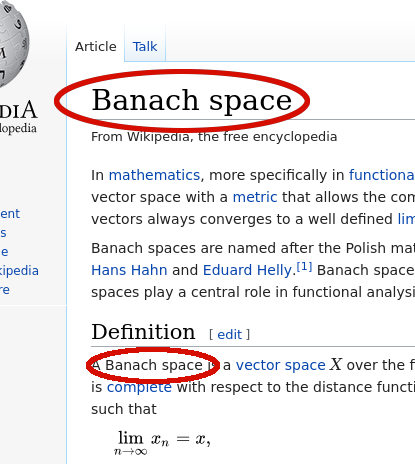
\includegraphics[width=0.9\textwidth]{../Images/wiki_thin_banach.png}
        \end{column}
        \pause
        \begin{column}{0.6\textwidth}
            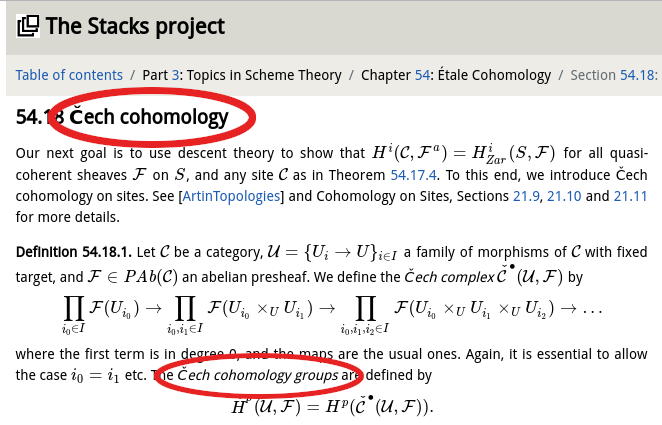
\includegraphics[width=0.8\textwidth]{../Images/stacks_defs.png}
        \end{column}
    \end{columns}

\end{itemize}
\end{frame}


%%%%  FRAME  %%%%
\begin{frame}
    \frametitle{Finetuning a Pretrained Model}
    Using this data we can train a \textbf{text classifier} (Sequence Classifier). To find all paragraphs that ``\textit{look}'' like a definition (Ginev 19). \pause From \textcolor{blue}{arxiv.org/abs/0805.2034}
    \begin{center}
        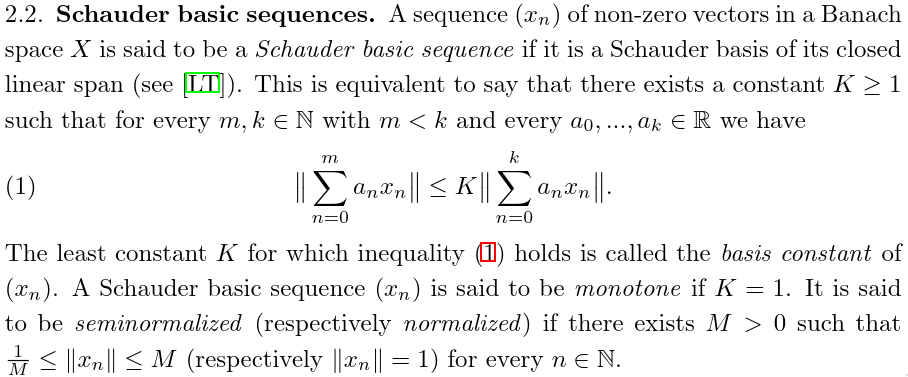
\includegraphics[width=0.7\textwidth]{../Images/def2.png}
    \end{center}
    \phantom{After this, we train a \textbf{token classifier}, to find the term that is being defined.}
\end{frame}

%%%%  FRAME  %%%%
\begin{frame}
    \frametitle{Finetuning a Pretrained Model}
    Using this data we can train a \textbf{text classifier} (Sequence Classifier). To find all paragraphs that ``\textit{look}'' like a definition (Ginev 19). From \textcolor{blue}{arxiv.org/abs/0805.2034}
    \begin{center}
        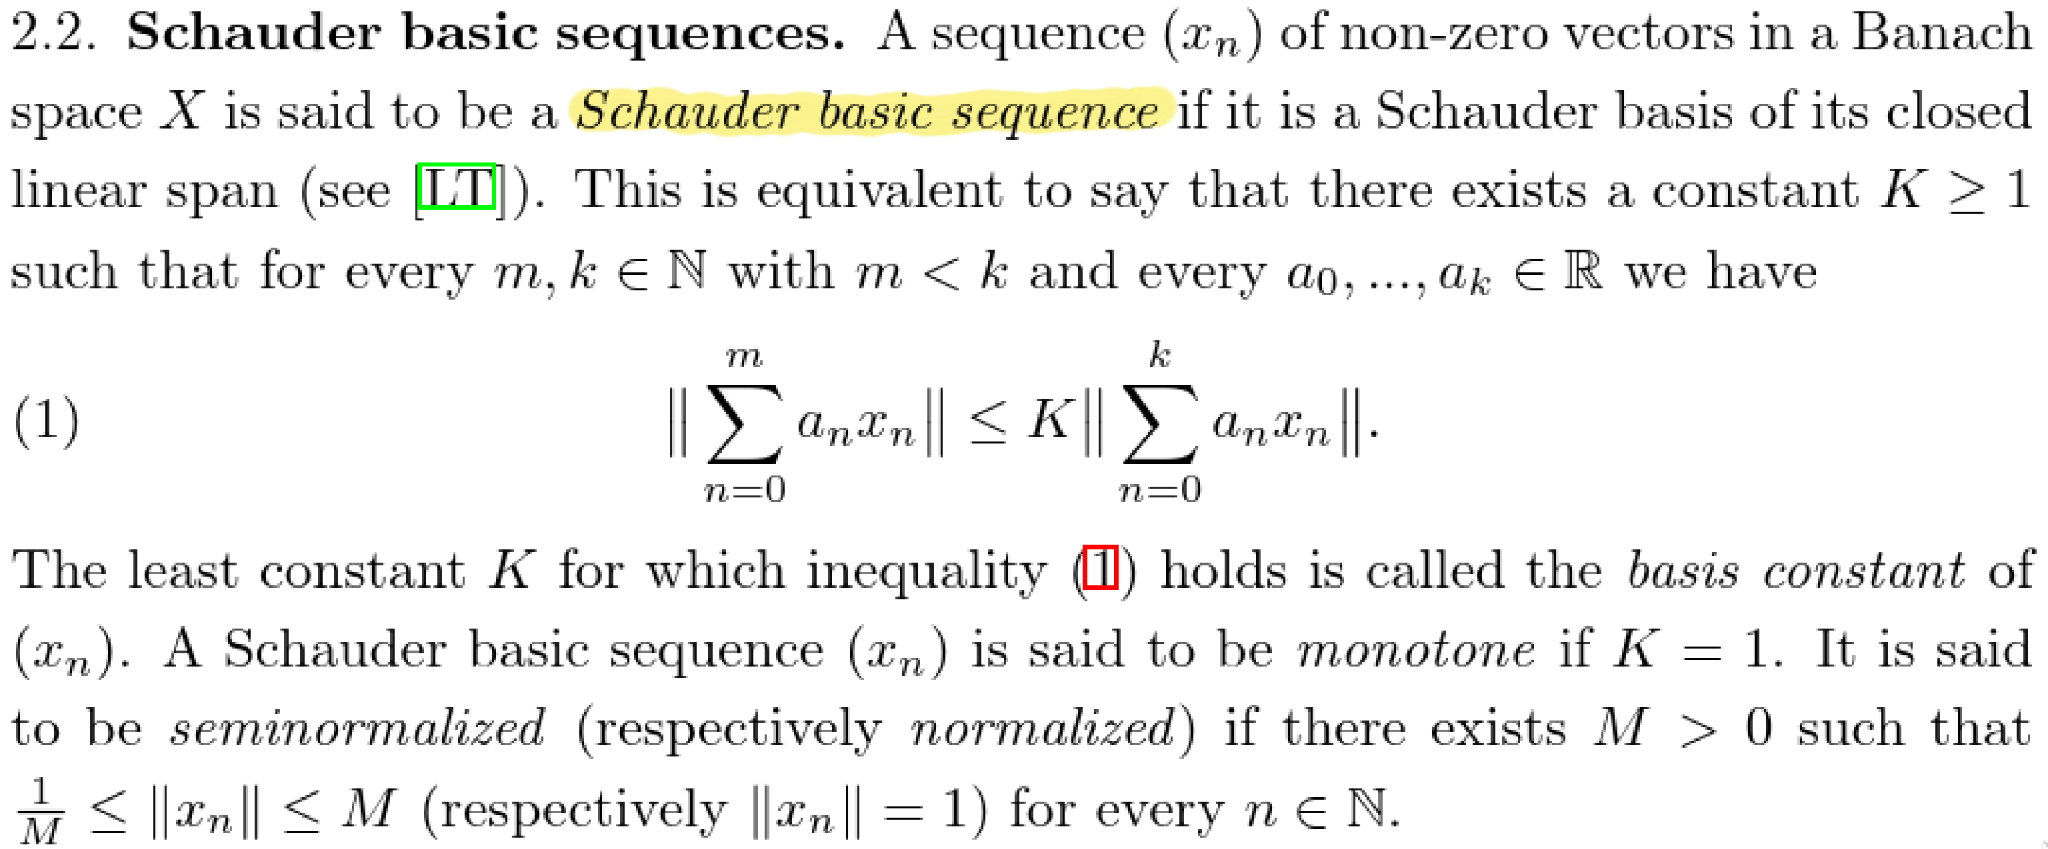
\includegraphics[width=0.7\textwidth]{../Images/def_highlighted.png}
    \end{center}
 After this, we train a \textbf{token classifier}, to find the term that is being defined.
\end{frame}

%%%%  FRAME  %%%%
\begin{frame}[containsverbatim]
    \frametitle{Code Example}
    \framesubtitle{Finetuning a pre-trained model.}
    \begin{minted}{python}
# IMPORT HUGGINGFACE LIBRARIES
from transformers import (AutoTokenizer,
                  AutoModelForSequenceClassification,
                  TFAutoModelForTokenClassification,
                  DataCollatorWithPadding,)

#checkpoint = "roberta-large"
#checkpoint = "bigscience/bloom-1b1"
checkpoint = "gpt2"

# NUMBER OF ITERATIONS (3 - 5)
for epoch in tqdm(range(epochs)):
    train_labels, train_predict, train_loss = \
    train(train_dataloader,
        optimizer, scheduler, device)
    ... ... ...
    \end{minted}
\end{frame}

%%%%  FRAME  %%%%
\begin{frame}
    \frametitle{Main Metrics and Results}
    \begin{columns}
        \begin{column}{0.7\textwidth}
            \begin{center}
                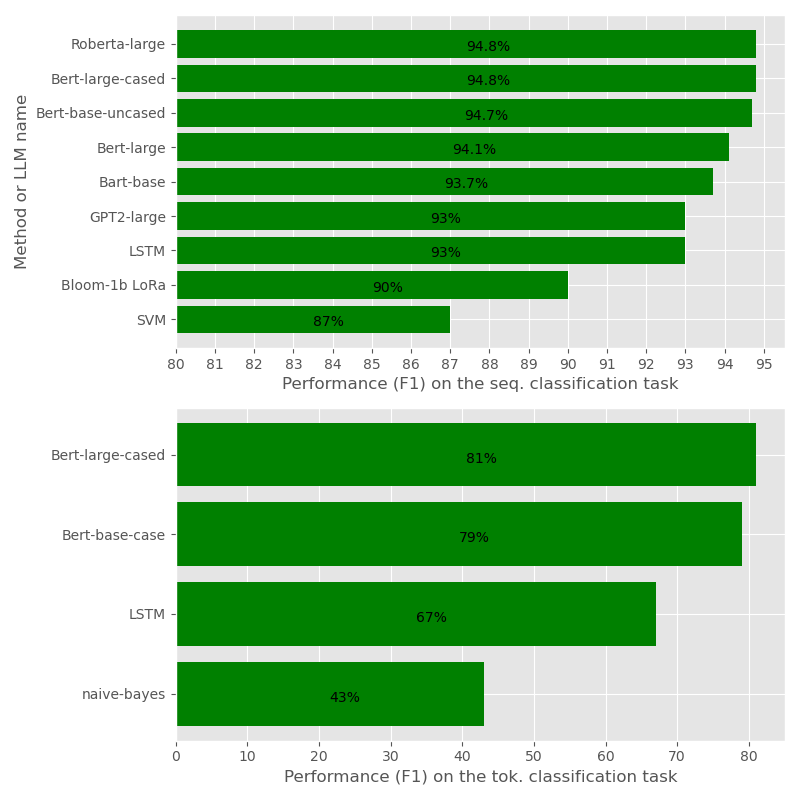
\includegraphics[width=0.9\textwidth]{../Images/taskbars.png}
            \end{center}
        \end{column}
        \begin{column}{0.3\textwidth}
            \begin{itemize}
                \item LLM's performance is better than neural and BOW-methods
                    \pause
                \item BERT had the best performance.
            \end{itemize}
        \end{column}
    \end{columns}
\end{frame}

%%%%  FRAME  %%%%
\begin{frame}
    \frametitle{A look at the Results}
    \begin{columns}
        \begin{column}{0.4\textwidth}
            Terms with multiple words only \\
            \begin{tabular}{lr}
                \toprule
                \textbf{Term} & \textbf{\#}  \\
                \midrule
full subcategory &  6,836 \\
weak solution &  4,926 \\
finitely generated &  3,791 \\
well defined &  3,476 \\
tensor product &  2,937 \\
simplicial complex &  2,610 \\
lie group &  2,578 \\
finite set &  2,341 \\
probability measure &  2,089 \\
banach space &  2,027 \\
borel measure &  1,999 \\
young diagram &  1,985 \\
non degenerate &  1,861 \\
moduli space &  1,848 \\
hilbert space &  1,795 \\
\bottomrule
            \end{tabular}
        \end{column}
        \begin{column}{0.6\textwidth}
            \begin{center}
                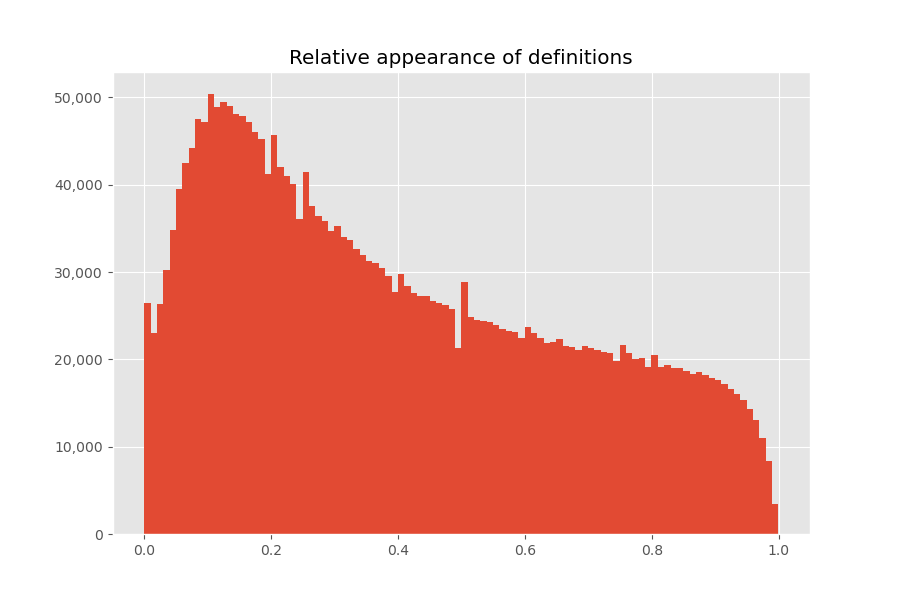
\includegraphics[width=0.95\textwidth]{../Images/rel_appe.png}

                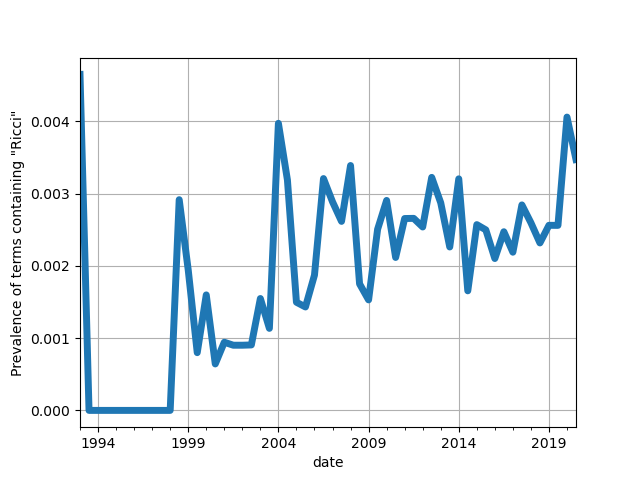
\includegraphics[width=0.85\textwidth]{../Images/ricci_preval.png}
            \end{center}
        \end{column}
    \end{columns}
\end{frame}



%%%%  FRAME  %%%%
\begin{frame}
    \frametitle{Organizing the Terms by Similarity}
    \framesubtitle{With word embeddings and cosine similarity}
            \begin{figure}
                \centering
                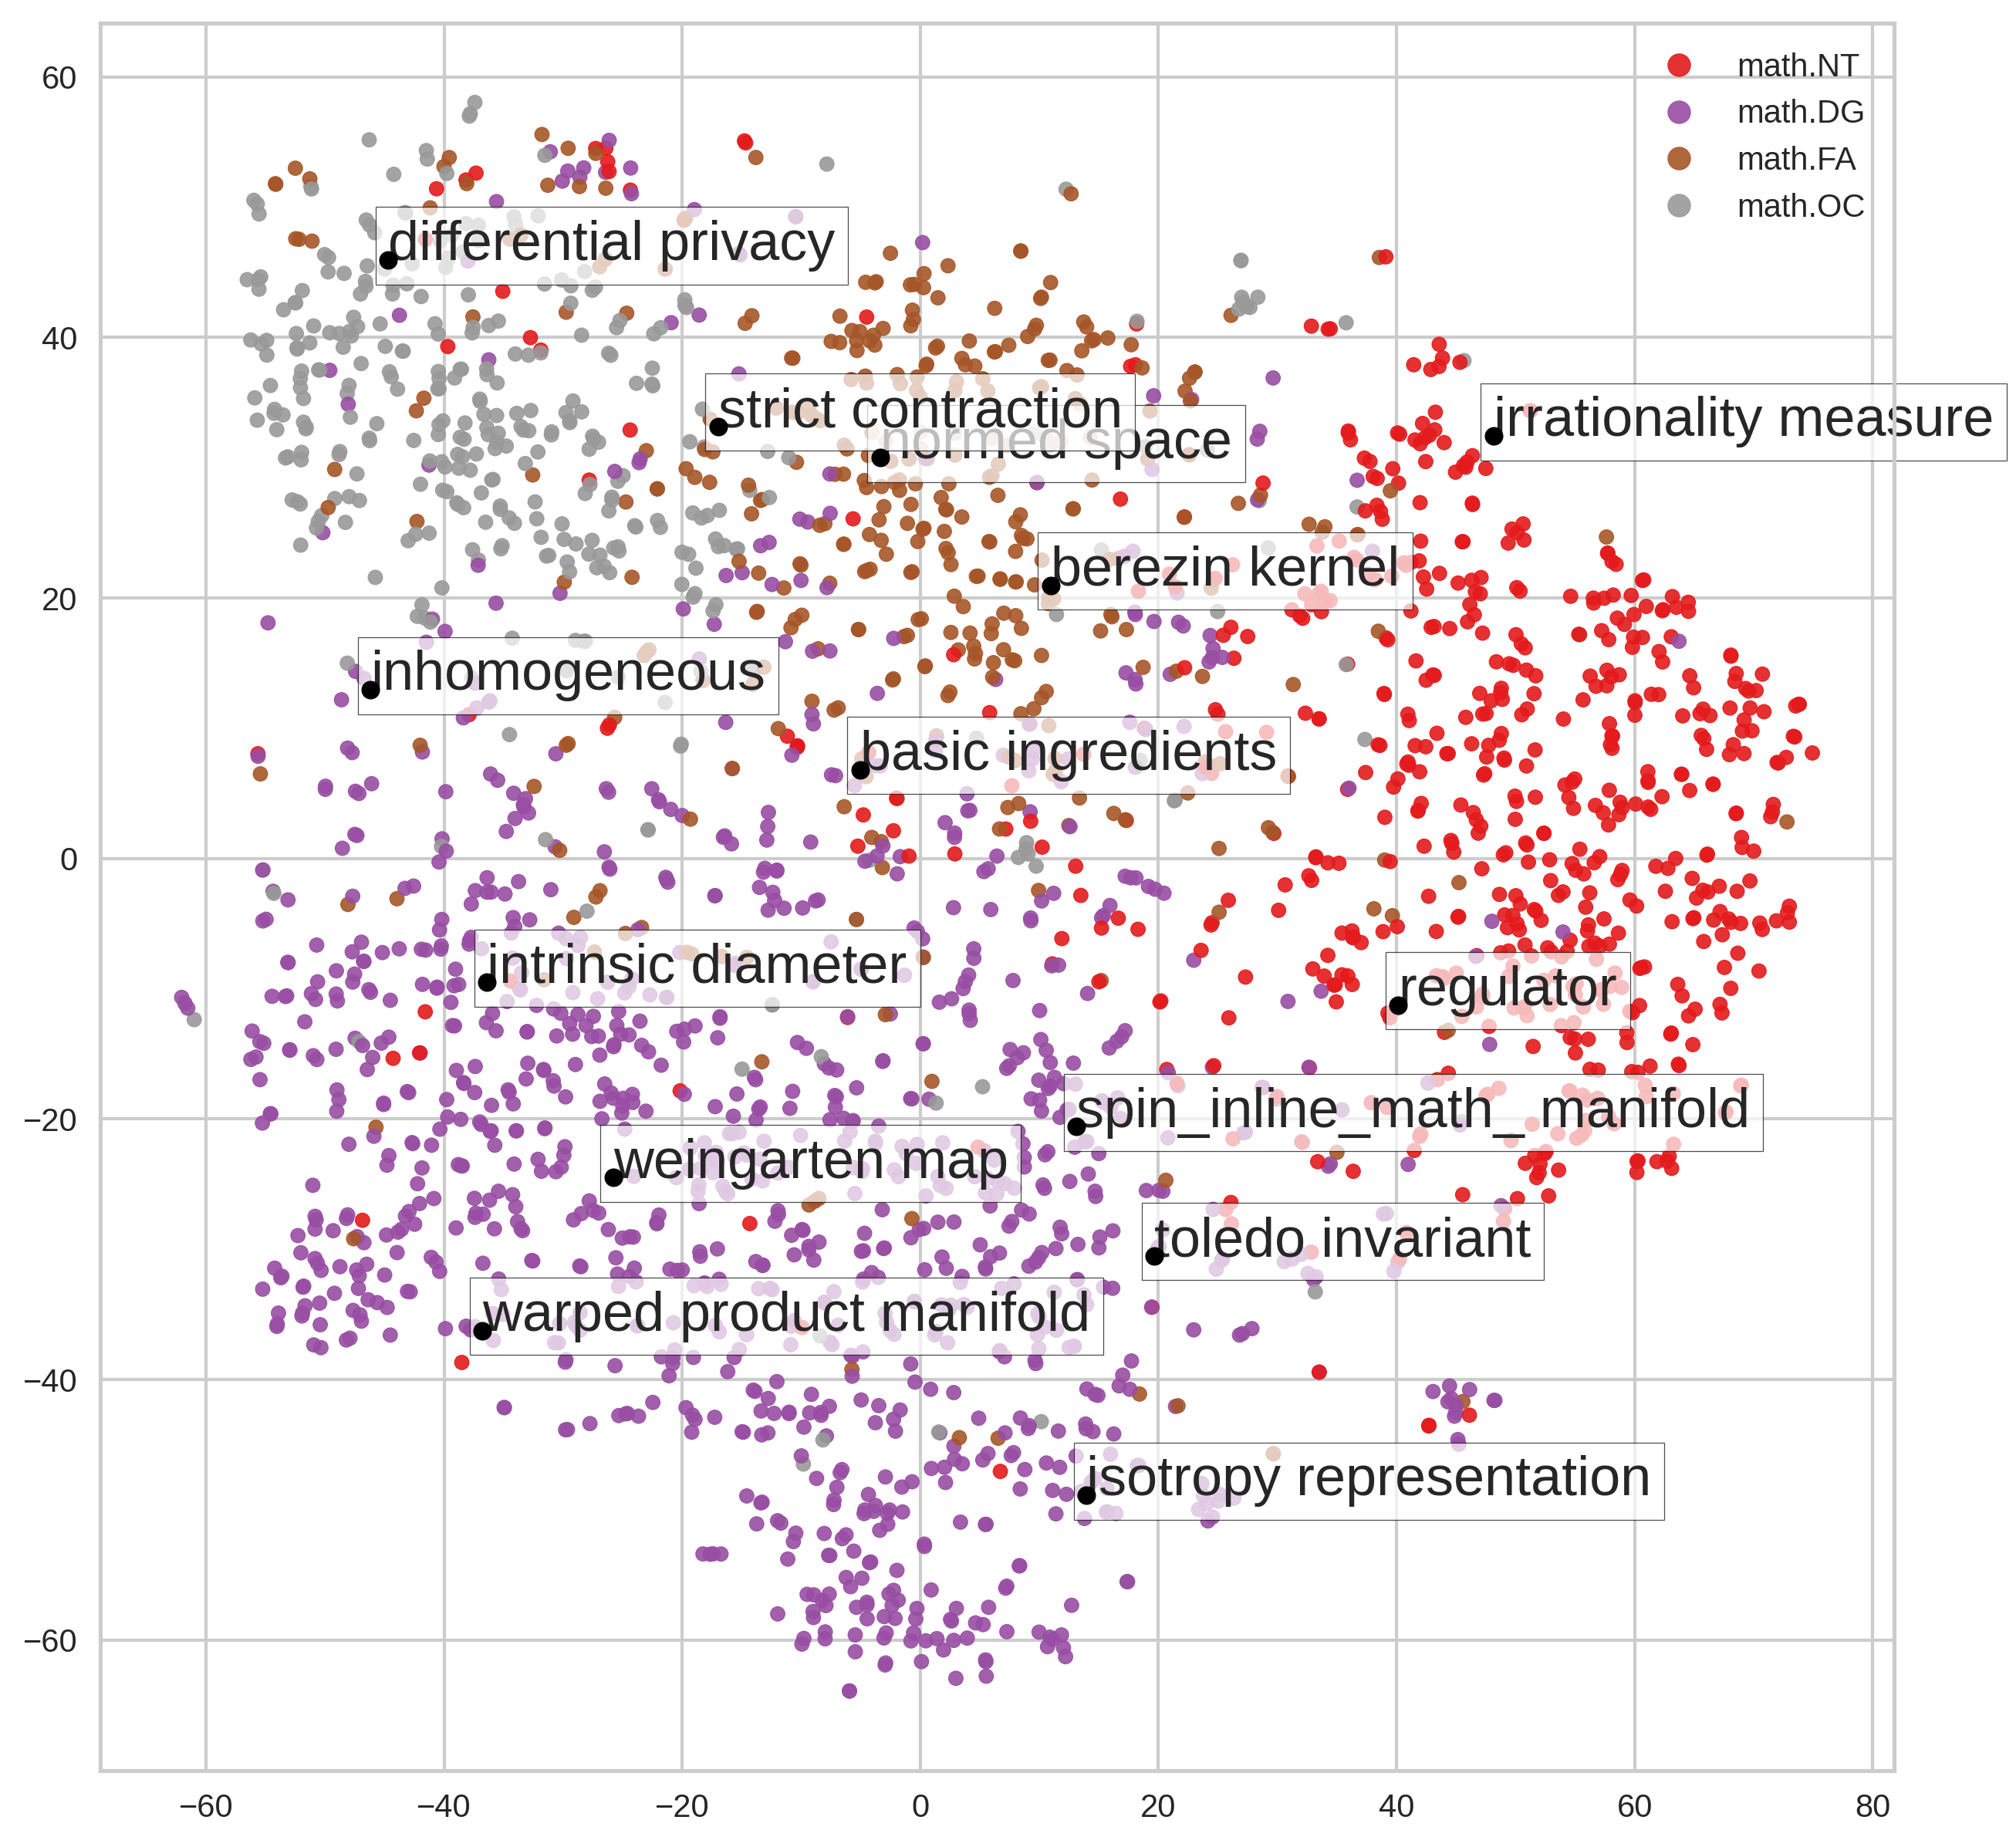
\includegraphics[width=0.9\textwidth]{../Images/scatter_option5.png}
            \end{figure}
\end{frame}

%%%%  FRAME  %%%%
\begin{frame}
    \frametitle{Organizing the Terms by Similarity}
    Nearest Neighbors gives 
            \begin{figure}
                \centering
                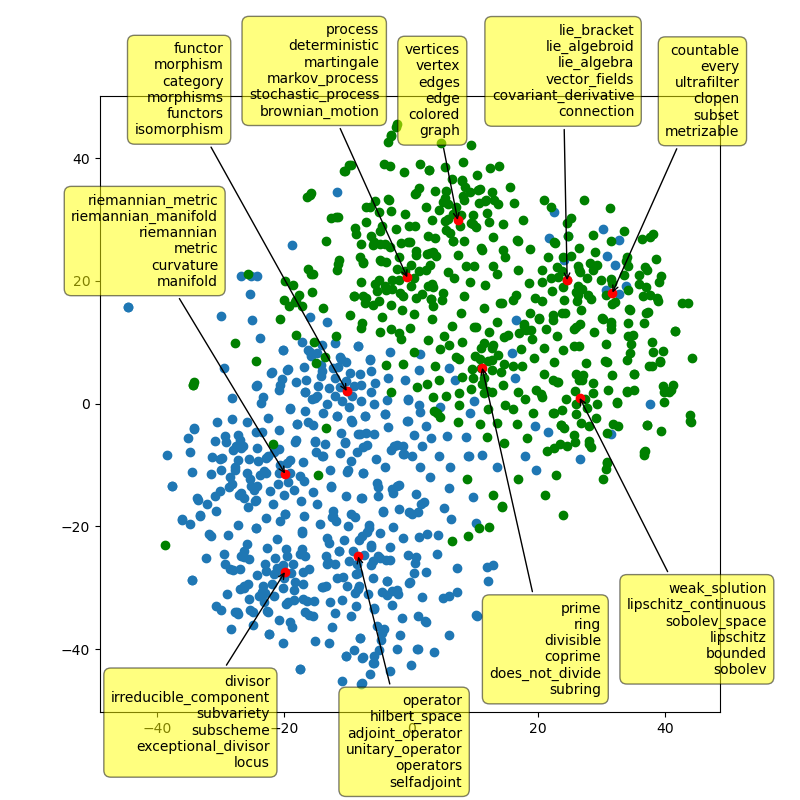
\includegraphics[width=0.75\textwidth]{../Images/showcenters.png}
            \end{figure}
\end{frame}

%%%%  FRAME  %%%%
\begin{frame}
    \frametitle{Organizing the Terms by Dependency}
    \begin{itemize}
        \item We can estimate the variance of a term, how diverse its usage is. \pause
        \item Together with the mean gives a point in the upper half-plane model of hyperbolic geometry (Costa 2015).
            \pause
        \item It can be said for terms that are nearby, that higher terms depend on lower ones: The \textbf{is-a} score (Tifrea 2018)
            \pause
            \begin{tabular}{rclr}
                \centering
hausdorff\_space & \textbf{is-a}  &   topology  &  0.4556 \\
minimal\_polynomial & \textbf{is-a} & characteristic\_polynomial  &  0.2699 \\
ufd   & \textbf{is-a}   &      pid &  -0.3642 \\
commutative\_ring & \textbf{is-a} & integral\_domain  & -0.5173 \\
\end{tabular}
\pause
\item It does not work when the terms have more than one meaning.
            \begin{tabular}{rclr}
                \centering
ufd  & \textbf{is-a}  & field  & 2.2690 \\
\end{tabular}
    \end{itemize}
\end{frame}

%%%%  FRAME  %%%%
\begin{frame}
    \frametitle{Alignment with Libraries}
            \begin{figure}
                \centering
                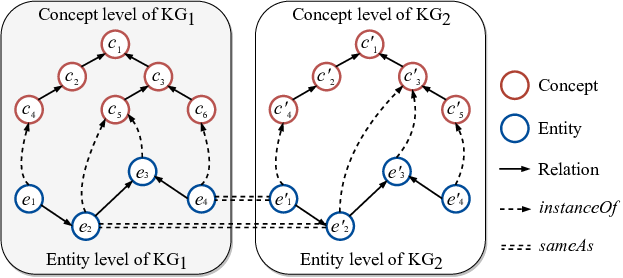
\includegraphics[width=0.5\textwidth]{../Images/example.png}
                \caption{Zequn Sun and Muhao Chen, Knowledge Association with Hyperbolic Knowledge Graph Embeddings}
            \end{figure}
\end{frame}

%%%%  FRAME  %%%%
\begin{frame}
    \frametitle{Generating a Knowledge Graph}
    Searching for Nearest Neighbors and sorting by \textbf{is-a} score. Gives a dependency graph.
            \begin{figure}
                \centering
                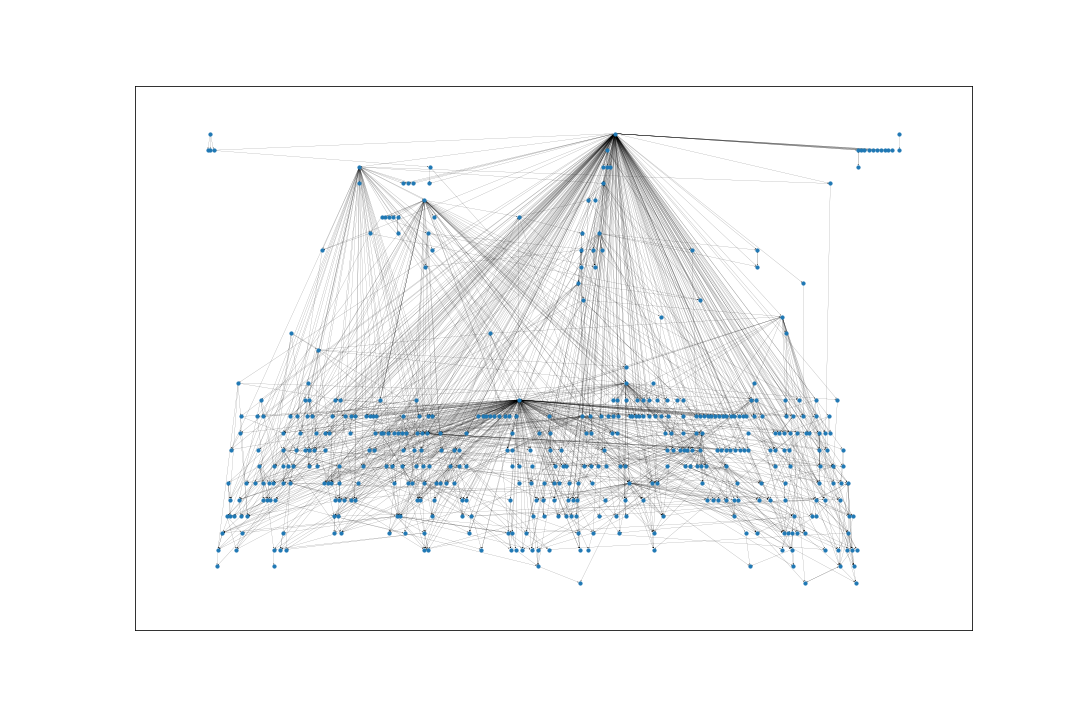
\includegraphics[width=0.99\textwidth]{../Images/number_theory_dgraph.png}
            \end{figure}
\end{frame}


%%%%  FRAME  %%%%
\begin{frame}
    \frametitle{WIP: Alignment with Formal Libraries}
    \begin{itemize}
        \item This can be used to associate entities in different knowledge graphs in the following way:
            \pause
        \item Given a few number of identified nodes in each graph. We can find the best transformation from KG$_1$ to KG$_2$. For example, 
            the \texttt{HyperKA} (Sun 2020)
    \end{itemize}
            \begin{figure}
                \centering
                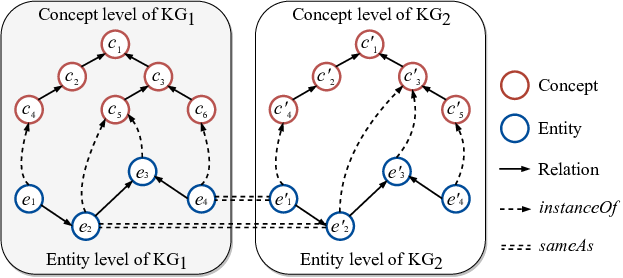
\includegraphics[width=0.5\textwidth]{../Images/example.png}
                \caption{Zequn Sun and Muhao Chen, Knowledge Association with Hyperbolic Knowledge Graph Embeddings}
            \end{figure}
\end{frame}

%%%%  FRAME  %%%%
%\begin{frame}
%    \frametitle{Future Work}
%    \begin{itemize}
%        \item Usar Zero-shot o RAG con los modelos más grandes.
%            \note{Aunque no puede afinar (finetune) modelos de $\geq$ 70B de parametros,}
%            \pause
%        \item Esperar el ``port'' de modelos de Huggingface a Neocortex.
%            \pause
%        \item Dejar de usar preprocesadores del código fuente de \LaTeX{}.
%    \end{itemize}
%\end{frame}


%%%%  FRAME  %%%%
\begin{frame}
    \frametitle{Conclusions}
    \begin{itemize}
        \item This approach  generates a comprehensive list of terms and definitions.
        \item Provides fast search results for internal and possibly external relationship of similarity and dependency.
        \item Really interested about possible applications to flexiformal documents or the tetrapod model.
    \end{itemize}
\end{frame}

\begin{frame}
\titlepage
\end{frame}
\end{document}
